\documentclass[12pt]{article}
\usepackage{listings}
\usepackage[colorlinks=true,pagebackref,linkcolor=blue]{hyperref}
\textwidth=7in
\textheight=9.5in
\topmargin=-1in
\headheight=0in
\headsep=.5in
\hoffset  -.85in

\lstset{
basicstyle=\footnotesize\ttfamily,
language=bash,
upquote=true,
breakatwhitespace=true,
columns=fullflexible,
keepspaces,
%numbers=none,
tabsize=3,
frame=blrt,
framextopmargin=5pt,
showstringspaces=false,
extendedchars=true
}

\pagestyle{empty}

\renewcommand{\thefootnote}{\fnsymbol{footnote}}
\usepackage{graphicx}
\begin{document}



\begin{center}
{\bf AMS 550.400 \quad HW SET 1\quad  Due Date:  Oct 8}\\
\vskip.2in
{\footnotesize Last Compiled on \today}
\end{center}

\setlength{\unitlength}{1in}

\begin{picture}(6,.1) 
\put(0,0) {\line(1,0){6.25}}         
\end{picture}

 

\renewcommand{\arraystretch}{2}

\vskip.25in
\noindent\textbf{Problem 1 (10 pts):}  

\vskip.25in
\begin{enumerate}
\item mkdir hw1p1.git 
\item cd hw1p1.git 
\item git init . 
\item vi main.txt
\item git add .
\item git commit -m "A added to master"
\item vi main.txt
\item git add .
\item git commit -m "B added to master branch"
\item git branch alt
\item git branch
\item vi main.txt
\item git add .
\item git commit -m "C added to master branch"
\item git checkout alt
\item vi main.txt
\item git add .
\item git commit -m "X added to alt branch"
\item git checkout master
\item git merge alt
\item vi main.txt
\item git add .
\item git commit -m "Alt merged to master branch"
\item git branch
\item vi main.txt
\item git add .
\item git commit -m "D added to master branch"
\item git log --graph --oneline
\item git checkout alt
\item git log --graph --oneline
\end{enumerate}

\begin{figure}[h]
    \begin{center}
        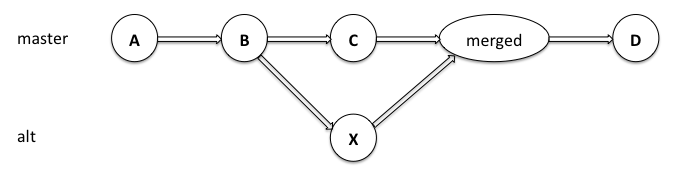
\includegraphics[width=\textwidth]{master_commitgraph.png}
    \end{center}
    \caption{Master Commit Graph}
    \label{fig:mcg}
\end{figure}

\begin{figure}[h]
    \begin{center}
        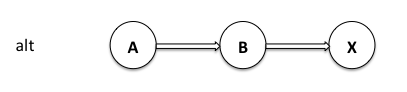
\includegraphics[width=\textwidth]{alt_commitgraph.png}
    \end{center}
    \caption{Alt Commit Graph}
    \label{fig:acg}
\end{figure}

\begin{picture}(6,.1) 
\put(0,0) {\line(1,0){6.25}}         
\end{picture}

\vskip.25in
\noindent\textbf{Problem 2 (10 pts):}

\vskip.25in
\begin{enumerate}
\item mkdir hw1p2.git
\item cd hw1p2.git
\item git init .
\item git remote add s1 git://github.com/nhlee/550400.stanza1.git
\item git pull s1 master
\item vi main.txt
\item git add .
\item git commit -m "Title added"
\item git remote add s2 git://github.com/nhlee/550400.stanza2.git
\item git pull s2 master
\item vi main.txt
\item git add .
\item git commit -m "2nd stanza merged"
\item git remote add s3 git://github.com/nhlee/550400.stanza3.git
\item git pull s3 master
\item vi main.txt
\item git add .
\item git commit -m "3rd stanza merged"
\item git remote add origin https://github.com/tangdnn/550400.homeworkset.1.git
\item git push origin master
\item git remote rm origin
\end{enumerate}

\begin{picture}(6,.1) 
\put(0,0) {\line(1,0){6.25}}         
\end{picture}

\vskip.25in
\noindent\textbf{Problem 3 (40 pts):}

\vskip.25in
For this exercise, we wish to build a cooperative strategy for a team of four students who have split up the presentation into four parts. 
\vskip.15in
\noindent\textbf{Strategy 1:}
\begin{itemize}
\item \textbf{Formulate the Problem.} Since they do not wish to work concurrently, we must develop a work flow strategy for the team to merge all four parts together without the need for a group meeting using \texttt{git}. 
\item \textbf{Outline the Model.} One work flow strategy for this team is to for the team members to merge their presentation consecutively; i.e.: \emph{B} merge with \emph{A}, then \emph{B} merge with \emph{C}, and lastly, \emph{D} merge with \emph{C}. The endogenous variable of this model is for all four team members to combine their respective parts of the presentation without working concurrently during a group meeting. The exogenous variable of this model is an effective work flow strategy proposal---in this case, merging each part consecutively using \texttt{git}---to combine different parts of the presentation. Unimportant variables that can be neglected are the amount of time it takes to write each part on its own (assuming that at least two parts are done at the time of merging), the physical quantity of each part, and the consistency of each students' writing. In this case, the combination of all four parts of the presentation (endogenous variable) depends on the process of consecutive merging work flow strategy (exogenous variable).
\item \textbf{Is It Useful?} Yes, the consecutive merging work flow model is useful. The model fulfills all of the requirements set by the problem. Since model requires \emph{B}, \emph{C}, and \emph{D} to merge each previous part, the actual merging does not require any group members to be present, least of all at the same time. The merging can be done on team member's own time. More importantly, this strategy allows all four parts to be merged in \texttt{git}. 
\item \textbf{Test the Model.} We can predict that this model is efficient. Since the whole model can be done in very quickly, assuming that all students have their respective parts done at the time of merging, we can say that the model is efficient. We can also test that this model can be done quickly. Even if not all students have their parts done at the same time, each merging step would only take a minute or two. Thus, we can say that this model can also be done quickly. 
\item \textbf{Strengths and Weaknesses.} The advantages of this model is that it allows the team members to combine their parts of the presentation together without needing them to be present at the same time. The model is also quick and efficient, as explored in the Test the Model section. However, one major disadvantage is that since there is no requirement for all students to have their parts done at the same time, each merging step might be delayed since it depends on whether or not one of the students finished their part. The model might be held up if \emph{A} did not finish the \emph{Introduction}, and students \emph{B}, \emph{C}, and \emph{D} have to wait for \emph{A} to finish in order to combine the presentation.
\end{itemize}

\vskip.25in
\noindent\textbf{Strategy 2:}
\begin{itemize}
\item \textbf{Formulate the Problem.} Like the previous model, the problem remains the same. We must develop a \emph{different} work flow strategy for the team to merge all four parts together without the need for a group meeting using \texttt{git}. 
\item \textbf{Outline the Model.} Another work flow strategy for this team is for all team members to push their \texttt{git} folders to a shared \texttt{git} repository and then for one group member to pull the contents of that repo and merge all four parts manually. Like the previous strategy, the endogenous variable of this model is for all four team members to combine their respective parts of the presentation without working concurrently during a group meeting. The exogenous variable of this model is the proposed work flow strategy---in this case, pushing four \texttt{git} folders to the same \texttt{git} repo and for one group member to pull the contents and merge the four parts together. Unimportant variables that can be neglected are the amount of time it takes for each students to write their part (since we are assuming that all parts are done at the time of merging), the physical quantity of each part, and the consistency of the students' writing. Like the previous strategy, the combination of all parts of the presentation (endogenous variable) depends on the simultaneous merging work flow strategy (exogenous variable).
\item \textbf{Is It Useful?} Yes, the simultaneous merging work flow model is useful. The model fulfills all requirements set by the problem. Since the merging process is done by only one student, none of the team members need to meet at a group meeting to combine the presentation. Lastly, the model allows the presentation to be merged using \texttt{git}.
\item \textbf{Test the Model.} To test this model, we can predict that the model is efficient. Assuming that the students have pushed their respective parts to the \texttt{git} repo at the time of merging, the whole model can be done soon after all parts are present in the repo. Thus, we can say that the model is efficient. 
\item \textbf{Strengths and Weaknesses.} The advantage of this model is that it allows team members to combine their parts of the presentation together without needing them to be present at the same time. This model is also efficient, as explored in the Test the Model section. One major disadvantage is similar to the previous model; the student doing the merging step might be waiting on all the other students to push their folder to the \texttt{git} repo, and it might be delayed if not all parts are present in the repo. Additionally, this model forces one group member to take on extra work for the project, which results in unfair distribution of work.
\end{itemize}
\vskip.25in
\noindent\textbf{Final recommendation:} We should use Strategy 1 for this presentation, since it has less disadvantages and more advantages than Strategy 2. It allows a more fair distribution of work and efficient process. 

\begin{picture}(6,.1) 
\put(0,0) {\line(1,0){6.25}}         
\end{picture}

\vskip.25in
\noindent\textbf{Problem 4 (aka.\ Fair Play, 40 pts):}
\vskip.25in
To answer this question, we must first be familiar with the rules of tennis and to be able to define 'fair game.' A fair game is a game, whether athletic or academic, where all the contestants have the same chance of winning. In tennis, a fair tennis game is a game where both players have an equal chance of winning. However, one aspect of tennis seems to contradict the definition of 'fair game': One player will be serving the ball, which is assumed to be more advantageous than receiving the ball. We hope to explain this using a mathematical model.

\vskip.25in
\begin{itemize}
\item \textbf{Formulate the Problem.} In tennis, serving the ball is assumed to be more advantageous than receiving the ball, since players can use the serve to put more offensive power into the serve. Furthermore, the server has less chance to lose the set since they served the ball first. The problem we are looking to investigate is to determine if a tennis game is fair (i.e.: if serving the ball really does give the server an advantage over the receiver).
\item \textbf{Outline the Model} For this model, we will need to simplify many factors. Since it is far too complex to realistically model a game of tennis, we will only take a few things into account. Firstly, we cannot incorporate the players' physiological and mental states into the model. It will be difficult to realistically include these factors, even if they can seriously impact the outcome of the game. We must assume that both players are at the same mental and physiological states. Secondly, we assume that both players are at the same skill level; if one player is obviously better at tennis than the other, then the 'fair game' model will be obselete. Thirdly, we assume that both players maintain the same level of play for the whole game. None of the players will unexpectedly change their style of play in the middle of the game or adapt to the other player's style of play. These factors ensure that the tennis game is more fair. 
\vskip.15in
Suppose we say that serving does give the server an advantage over the receiver with a probability \emph{p} of winning the game, where \emph{p} is greater than or equal to 0.5. Thus, the receiver has a probability \emph{(1-p)} of winning the game. Assuming that there are \emph{n} games in a set, where \emph{n} is even and greater than or equal to 6; one player must win by 2 games, and must play at least 6 games to win a set. 
\vskip.15in
The endogenous variable in this model is the fairness of the tennis game. The exogenous variables in this model are similar to the assumptions we made: the physiological and mental states of the tennis players, the skill levels of the players, and the consistency of their style of player. Unimportant factors of this model are the time of day, playing equipment, and the presence of an audience. The fairness of the tennis game (endogenous variable) depends heavily on the assumptions that we made (exogenous variables).
\item \textbf{Is It Useful?} Yes, the 'fairness' model is useful. By assuming that all factors are equal for both players during the tennis game, we ensured that the model is fair. By taking into account of the serving advantage, we also modeled the part of the problem that we wished to investigate. Thus, we can say that the model is accurate (for our purposes) and useful.
\item \textbf{Test the Model} We predict that the tennis game is fair based on the model we made. Since there are \emph{n} number of games in the set, we can assume that the serving advantage will even out over a large number of games, and thus the probability of winning the set will also even out over a large number of games. Since the server and receiver switch every game, the serving probability will cancel out in only 2 games. Using this test on the model, we can say that there is no serving advantage to the server, and that \emph{the game of tennis is fair.}
\end{itemize}

\end{document}
